\documentclass{beamer}



\colorlet{structure}{blue!65!white}

\beamertemplateshadingbackground{black!50}{white}



%\mode<presentation>
%{ \usetheme{boxes} }

\usepackage{beamerthemesplit}
\usepackage{graphics}
\usepackage{graphicx}
\usepackage{verbatim}
\usepackage{graphicx}

\title{Low Memory Graph Traversal}
\author[Samson Bassett]
{ 
Samson Bassett \\
Master of Science Defense\\
Simon Fraser University 
}
\date{August 23, 2010}


%\AtBeginSection[] %make this recurring outline show at each section
%{
%\begin{frame}<beamer>
%\frametitle{Outline}
%\tableofcontents[currentsection]
%\end{frame}
%}

\begin{document}

\frame{\titlepage}


\frame{ \frametitle{Outline} \tableofcontents}


%begin content slides

\section{Introduction}

\frame{\frametitle{Introduction}\begin{itemize}

  \item The graph traversal problem 
requires an algorithm that starts on an arbitrary vertex, and moves along edges to eventually 
visit every vertex of the graph. 
    \pause

    \item Trivial memory lower bound for graph traversal $\Omega(\log n)$.  We wish to achieve this lower bound whenever possible.
 \pause

\item Model of Computation is a Finite Automaton that only knows local information of the graph
\pause

\item There are two main classes of graphs, anonymous graphs and labelled graphs.
\end{itemize}}






\section{Periodic Traversal}

\frame{\frametitle{Anonymous Graphs}\begin{itemize}

\item A graph that does not have a unique label for every vertex is called an anonymous graph.
\pause

\item In anonymous graphs, we allow edges at an incident vertex to be distinguishable from one another, 
called a \emph{local orientation} of the graph, represented by port numbers

\end{itemize}}





\frame{\frametitle{Motivation}\begin{itemize}

\item \begin{theorem}\emph{(Fraigniaud et. al., 2005)} For any finite automaton with 
$K$ states, and any $d\ge 3$, there exists an anonymous planar graph $G$ of maximum degree $d$ with 
at most $K+1$ vertices that the finite automaton cannot traverse. \end{theorem}%fippp

\pause

\item What if the local orientation is not arbitrary?

\end{itemize}}




\frame{\frametitle{Definition}\begin{itemize}

%\item By constructing a specific local orientation for the graph, we can perform a Periodic Traversal

\item Periodic graph traversal requires that an algorithm visits every vertex 
infinitely many times in a periodic manner

\pause

\item The period of a traversal on a graph with $n$ vertices is the maximum number of edge traversals 
performed between two consecutive visits of a generic 
vertex, denoted by $\pi(n)$

\end{itemize}}

















\frame{\frametitle{Previous Results}\begin{itemize}

\item \begin{theorem}\emph{(Dobrev et. al., 2005)} If $G$ is an anonymous graph on $n$ 
vertices, there exists a local orientation and a corresponding robot (with $1$ state) that 
will periodically traverse $G$ with period $\pi(n)\le 10n$\end{theorem}

\item \begin{theorem}\label{it3}
\emph{(Ilcinkas, 2008)}  If $G$ is an anonymous graph on $n$ vertices, there is a local 
orientation and a robot (with $3$ states) that will periodically traverse $G$ with 
period $\pi(n)\le 4n-2$\end{theorem}

\item \begin{theorem}\emph{(G\c{a}sieniec et. al., 2008)}  If $G$ is an 
anonymous graph on $n$ there is a local orientation of $G$ and a robot (with $11$ states) 
that will periodically traverse $G$, with 
period $\pi(n)\le 3.75n-2$\end{theorem}

\end{itemize}}






\frame{\frametitle{Lower Bound}\begin{itemize}

\item If $G$ is anonymous graph on $n$ vertices, the lower bound of the period of any periodic traversal is $\pi(n)\ge 2n-2$ 
\item In particular, trees achieve this bound

\pause
\item We wish to find a class of graphs (other than trees) that achieves the lower bound of $2n-2$

\end{itemize}}



\frame{\frametitle{Classes of Graphs}\begin{itemize}

\item Let $G$ be a $P_3$-free graph with $\delta(G)\ge 2$
\pause

\item \begin{lemma}\label{lemclass}
Let $G$ be a graph with $n$ vertices such that $G$ is $P_3$-free.  Then either $G$ is $2$-connected, or 
$\Delta(G)=n-1$.
\end{lemma}

\end{itemize}}







\frame{\frametitle{Robot}\begin{itemize}

\item The robot (finite automaton) has only one state, and it traverses the graph simply by following increasing port numbers

\pause

\item The robot will start on any vertex $v$
\item Initially, the robot will leave $v$ on the edge with port $d(v)$
\item At each subsequent vertex $v$, if the robot enters $v$ on port $i<d(v)$, it will leave on the edge with port $i+1$
\item Similarly, if the robot enters $v$ on port $d(v)$, it backtracks along the same edge (with port $d(v)$)

\end{itemize}}







\frame{\frametitle{$\Delta(G)=n-1$}\begin{itemize}

\item Let $v$ be a vertex of degree $n-1$

\item Since $\delta(G)\ge 2$, $v$ has two neighbours $x$ and $y$ that are adjacent
\pause
\item The assignment of port numbers handles all vertices the same except for these three, as shown in the following example
\end{itemize}}



\frame{\frametitle{$\Delta(G)=n-1$}%\begin{itemize}


%\item make new figure for this labelling - on a new slide -also add to thesis (line 1071)
\begin{figure}[htp] 
\centering 
\resizebox{6cm}{!}{\includegraphics{starblank.pdf}} 
%\caption{cp } 
\end{figure} 

%\end{itemize}
}

\frame{\frametitle{$\Delta(G)=n-1$}%\begin{itemize}


%\item make new figure for this labelling - on a new slide -also add to thesis (line 1071)
\begin{figure}[htp] 
\centering 
\resizebox{6cm}{!}{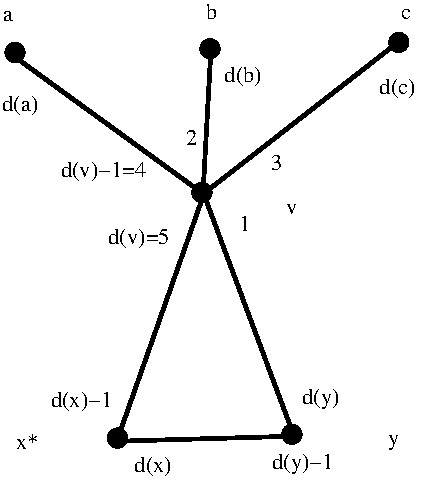
\includegraphics{starlab.pdf}} 
%\caption{cp } 
\end{figure} 

%\end{itemize}
}







\frame{\frametitle{$2$-connected graphs}\begin{itemize}
  

\item \begin{theorem}(Fleishner, 1974) If $G$ is $2$-connected, then $G^2$ has a Hamiltonian cycle \end{theorem}


\item Let $H$ be a Hamiltonian cycle of $G^2$ 
\pause
\item The main idea is to create a closed walk $H^*$ based on $H$ that visits every vertex of $G$ using only edges of $G$  
\item Then arrange port numbers so the robot will follow $H^*$ 
\item For our purposes, we will work with the \emph{symmetric orientation} of $G$ and $G^2$, denoted $\vec{G}$ and $\vec{G^2}$, respectively 

\end{itemize}}








\frame{\frametitle{$2$-connected graphs}\begin{itemize}

\item For every virtual edge of $H$, we assign a real path of length two, called a relay path 
\pause

\item If $P$ is a maximal virtual path in $H$ containing more 
than one vertex, such that all virtual arcs of $P$ share a common relay vertex $w$,  
then the subgraph $W$ of $\vec{G^2}$ consisting of $P$, and the relay path of every arc of $P$, is  
called a \emph{wedge}
\item The \emph{size} of $W$, denoted $s(W)$, is the number of vertices of $P$

\end{itemize}}


\frame{\frametitle{$2$-connected graphs}\begin{itemize}

\item We prove several lemmas related to wedges, the following describes how two wedges can interact
\item \begin{lemma}\label{lemwedge} Suppose $W_1$ and $W_2$ are distinct wedges.  Then \newline 

$(i)$  The wedges $W_1$ and $W_2$ have no virtual arcs in common.  \newline 
$(ii)$  The wedges $W_1$ and $W_2$ have no ribs in common.\newline   
%$(iii)$  If $e$ is a rib of $W_1$, $e^{-1}$ is not a rib of $W_2$.%mention this uses p3
\end{lemma} 

\end{itemize}}


\frame{\frametitle{$2$-connected graphs}

\begin{itemize}

%If $e$ is a backtrack arc of $v$, then $e$ is an isolated arc of $v$.
\item Given a vertex $v$, let $(x,v)$ and $(v,y)$ be the two arcs of $H$ incident with $v$.  
\pause
\item The incoming arc of $v$ is either   
$(x,v)$ if it is real, or the real arc $(w,v)$, where $w$ is the relay vertex of $(x,v)$
\pause
\item Similarly, the  
outgoing arc of $v$ is either $(v,y)$ if it is real, or  
the real arc $(v,w)$, where $w$ is the relay vertex of $(v,y)$. 
\pause
\item If $e$ is the incoming arc of $v$ and 
$e^{-1}$ is the outgoing arc of $v$, we say that $e$ is a backtrack arc of $v$, (in which case 
$e^{-1}$ is also a backtrack arc of $v$   

%\item incoming and outgoing arcs, followed by the lemma about a,b, tied wedges
\end{itemize}
}

\frame{\frametitle{$2$-connected graphs}

\begin{itemize}
\item The \emph{list of ordered wedges} $W_1,W_2,\ldots,W_k$ \emph{at} $v$  
is the ordered list of all wedges with the common relay vertex $v$ such that for $W_i$ and $W_j$ with $i<j$, the virtual path of $W_i$  
occurs before the virtual path of $W_j$ when following $H$ starting from $v$
\pause
\item There are a few technical lemmas that determine how this list of wedges at $v$ interact with the incoming and outgoing arcs of $v$
\item Using these we have five cases (subroutines) for the Port-Numbering procedure
\pause
\item We will fix $v$, and say $a$ is the incoming arc of $v$, and $b$ is the outgoing arc of $v$
\end{itemize}}


\frame{\frametitle{$2$-connected graphs}
%\centering 
%The arc $a$ is an isolated arc of $v$, and $b$ is not.
Assign $d(v)-s(W_1)$ to $a^{-1}$\newline
Assign $[d(v)-s(W_1)+1,d(v)]$ to $W_1$
%Assign $[d(v)-\sum_{i}s_i,d(v)-s_1-1]$ to $\{W_i\}_{i>1}$
%\begin{itemize}
%\centering 
\begin{figure}[htp] 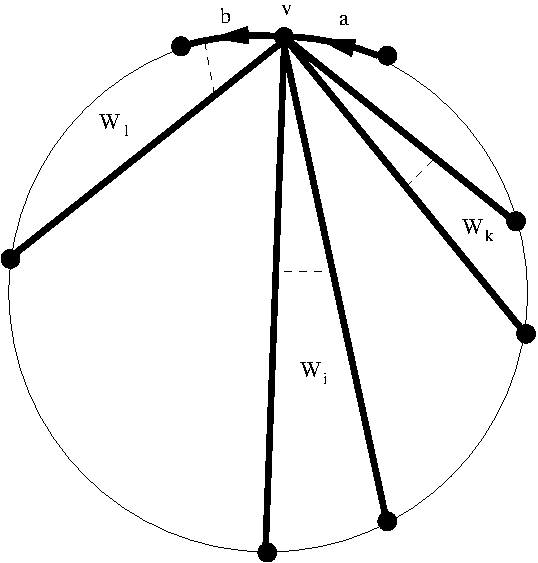
\includegraphics[width=4cm]{onlyaisoh.pdf} \end{figure}
\begin{center}The arc $a$ is an isolated arc of $v$, and $b$ is not.\end{center}
%\end{itemize}
}



\frame{\frametitle{$2$-connected graphs}

%\begin{itemize}
%\item spend a few slides on pictures and the labelling procedure 
   Assign   $[d(v)-s(W_{1}) +1 ,d(v)]$ to $W_{1}$\newline
   Assign  $[d(v)-s(W_{1})-s(W_{k})+1,d(v)-s(W_1)]$ to $W_{k}$
%\centering
\begin{figure}[htp] \resizebox{4cm}{!}{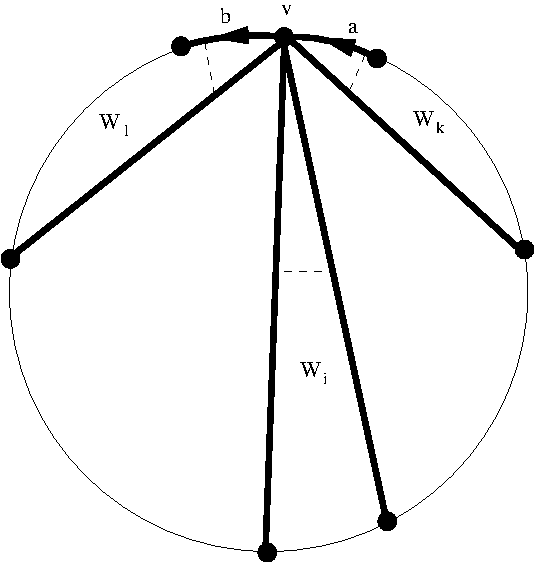
\includegraphics{noneiso.pdf}}\end{figure}
\begin{center}Neither $a$ nor $b$ are isolated arcs of $v$\end{center}
%\end{itemize}
}

%%%?????????????? if there is time, add a slide for the invariant?


\frame{\frametitle{Periodic Traversal Result}

\begin{itemize}
\item \begin{theorem}\label{pmain}
Let $G$ be a $P_3$-free graph, with $\delta(G)\ge 2$.  Then there exists a local orientation and a corresponding  
robot that will perform a periodic traversal 
of $G$ with period $\pi (n) \le 2n-2$ \end{theorem} 

\end{itemize}}

\frame{\frametitle{Future Work}\begin{itemize}


\item Drop the condition $\delta(G) \ge 2$ by adding a constant number of states to the robot
\item Create a procedure to assign ports for $P_3$-free graphs with $\delta(G)=1$
\pause
\item We conjecture that, using similar techniques as shown in this thesis, 
it is possible to create a local orientation (given some robot with a constant number of states) for $2$-connected graphs that are not $P_3$-free
%\item  for 
%some robot with a constant number of states

\end{itemize}}

\begin{comment}
\section{Graph Traversal Using Walks}

\frame{\frametitle{Definitions}\begin{itemize}


\item here we use labelled graphs ...show some negative results?
\begin{theorem}\label{l15}
\emph{\cite{NSW}}  Any labelled graph on $n$ vertices can be traversed in polynomial time and $O(\log^{1.5} n)$ memory.
\end{theorem}
\item ?.. define geometric graph
\end{itemize}}



\frame{\frametitle{Previous Results}\begin{itemize}

\item \begin{theorem}\emph{(de Berg et. al., 1997)}  Let $G$ be a geometric planar graph with $n$ vertices.  Then $G$ can be traversed 
in $O(n^2)$ time and $O(\log n)$ memory\end{theorem}

\begin{theorem}\emph{(Bose, Morin, 2002)}  Let $G$ be a geometric planar graph with $n$ vertices.  Then $G$ can be traversed 
in $O(n\log n)$ time and $O(\log n)$ memory\end{theorem} 

\item \begin{theorem}\emph{(Ch\'{a}vez et. al., 2004)}  Let $G$ be a graph 
with $n$ vertices that has a quasi-planar embedding that satisfies the Left-Neighbor Rule.  Then $G$ can be traversed 
in $O(m\log m)$ time and $O(\log n)$ memory\end{theorem}

\end{itemize}}




\frame{\frametitle{basic idea, covering and compatible order}\begin{itemize}

\item An oriented walk cover $W$ of $\vec{G}$ is a collection of closed walks from $\vec{G}$ such that 
each arc $e$ of $\vec{G}$ is in exactly one walk $w\in W$.  Furthermore, for any arc 
$e$ of $\vec{G}$, if $e\in w$, then $e^{-1} \notin w$.  We call $w$ a covering walk of $\vec{G}$
\pause
\item Let $G$ be an undirected graph, and suppose $\vec{G}$ has a total order on its arcs.  
We say this total order is compatible if for 
any arc $e$ of $\vec{G}$, there does not exist an arc $e'$ 
such that either $e<e'<e^{-1}$ or $e^{-1} < e' < e$
\end{itemize}}



\frame{\frametitle{list the main lemmas that are needed, virtual tree}\begin{itemize}


\item template

\end{itemize}}




\frame{\frametitle{result}\begin{itemize}


\item \begin{theorem}\label{thmc}
Let $G$ be a graph with $n$ vertices and $m$ edges.  Suppose that $G$ has an oriented walk cover, and 
$\vec{G}$ has a compatible total order on its arcs.  
Then the Walk-Traversal algorithm reports every edge of $G$ exactly once 
using $O(m \log m)$ time and 
$O(\log n)$ memory. 
\end{theorem}

\end{itemize}}




\frame{\frametitle{conjecture to apply to embeddings}\begin{itemize}


\item template

\end{itemize}}

\end{comment}
\section{References}

\frame{\frametitle{References}\begin{itemize}

\item R. Fleischer.  The square of every two-connected graph is Hamiltonian.  \emph{Journal of Combinatorial Theory, Series B},  
\textbf{16}(1) 29--34 (1974) 

\item P. Fraigniaud, D. Ilcinkas, G. Peer, A. Pelc, D. Peleg.  Graph exploration by a finite automaton.  \emph{Theoretical 
Computer Science}, \textbf{345} 331--344 (2005)  %fippp

\item L. G\c{a}sieniec, R. Klasing, R. Martin, A. Navarra, X. Zhang.  Fast 
periodic graph exploration with constant memory.  \emph{J Computer and System Science}, 
\textbf{74}(5) 808--822 (2008) %gkmnz


\end{itemize}}




\end{document}
